\chapter{Interfaces: HTTP API, Command Line and Demo}
\label{ch:interfaces}

Three interfaces sit on top of one \code{Pipeline} class. None of them contains retrieval or generation logic of its own.

\begin{center}
\begin{tabularx}{\textwidth}{@{}>{\raggedright\arraybackslash}p{2.3cm}>{\raggedright\arraybackslash}p{3.6cm}>{\raggedright\arraybackslash}p{4.4cm}L@{}}
\toprule
\textbf{Interface} & \textbf{Entry point} & \textbf{Pipeline lifetime} & \textbf{Intended user}\\
\midrule
HTTP API & \code{uvicorn vidyarag.api.main:app} (Docker, \code{make serve}) & Built once at startup, closed at shutdown & Programs; \code{/v1/search} for an agent in a sibling project\\
CLI & \code{vidyarag <command>} & Built per command, closed at exit & The developer: ingestion, evaluation, one-off questions\\
Gradio demo & \code{python app/app.py} (Space, \code{make ui}) & Built on the first question, kept for the life of the process & Visitors to the public demo\\
\bottomrule
\end{tabularx}
\end{center}

All three keep one pipeline per process for the same reason, repeated in each module: the embedded Qdrant index takes an exclusive lock on its directory and cannot be opened twice, and loading the local models is slow \ev{src/vidyarag/api/routes\_v1.py:3-6}, \ev{app/app.py:71-76}.

\section{The HTTP API}
\label{sec:api}

\subsection{Application and lifecycle}

\begin{lstlisting}[language=Python]
@asynccontextmanager
async def lifespan(app: FastAPI) -> AsyncIterator[None]:
    settings = Settings()
    configure_logging(settings.log_level, settings.log_format)
    logger = get_logger("vidyarag.api")
    pipeline: Pipeline = build_pipeline(settings)
    app.state.pipeline = pipeline
    logger.info("api.startup", profile=pipeline.config.name, collection=settings.qdrant_collection,
                embedding_model=pipeline.config.embedding_model,
                generation_model=pipeline.config.generation_model)
    try:
        yield
    finally:
        pipeline.close()
        logger.info("api.shutdown")

def create_app() -> FastAPI:
    app = FastAPI(title="VidyaRAG", description=DESCRIPTION, version=__version__, lifespan=lifespan)
    app.include_router(v1_router)
    @app.get("/", include_in_schema=False)
    def root() -> dict[str, str]:
        return {"service": "vidyarag", "docs": "/docs", "query": "POST /v1/query"}
    return app

app = create_app()
\end{lstlisting}
\vspace{-4pt}{\raggedleft\ev{src/vidyarag/api/main.py:30-70}\par}

Closing on shutdown matters for the embedded index: \enquote{a process that exits without closing leaves a stale lock that blocks the next run} \ev{src/vidyarag/api/main.py:3-6}. Startup does not need a Gemini key --- the model client is created lazily on the first answer --- so a server with no key starts, reports healthy, and fails only on \code{/v1/query}.

\subsection{Endpoints}

\begin{longtable}{@{}>{\raggedright\arraybackslash}p{2.5cm}>{\raggedright\arraybackslash}p{4.2cm}>{\raggedright\arraybackslash}p{4.9cm}>{\raggedright\arraybackslash}p{3.7cm}@{}}
\toprule
\textbf{Endpoint} & \textbf{Request} & \textbf{Response} & \textbf{Errors raised in code}\\
\midrule
\endhead
\code{POST /v1/query} & \code{question} (1--2,000 characters); \code{book_slug} (optional, \textbf{ignored}) & \code{answer}, \code{grounded}, \code{citations[]}, \code{context[]}, \code{trace} & \code{ValueError} (for example no API key) $\rightarrow$ 503; anything else $\rightarrow$ 500\\
\code{POST /v1/search} & \code{query} (1--2,000), \code{top_k} (1--20, default 5), \code{book_slug}; unknown fields rejected & \code{results[]}: chunk id, text, citation, book, chapter, section, printed page, source URL, score & Any exception $\rightarrow$ 503 \enquote{Retrieval failed: <type>}\\
\code{GET /v1/health} & --- & \code{status}, \code{collection}, \code{points}, embedding and generation model, \code{profile} & None\\
\code{GET /v1/config} & --- & Profile, description, models, embedding size, chunking, top-$k$ values, three retrieval flags, \code{corrective_enabled} & None\\
\code{GET /} & --- & Service name and links (hidden from the schema) & None\\
\bottomrule
\end{longtable}

\begin{measured}[the API served locally with the working index]
\code{POST /v1/query} returned 200 with an answer and two citations; \code{POST /v1/search} returned 200 with three hits; \code{GET /v1/health} reported 3,608 points; \code{/docs} returned 200; \code{/health} without the \code{/v1} prefix returned 404. The generated OpenAPI document is version 3.1.0, reports the API version as 1.2.1, and declares only 200 and 422 responses: the 503s raised in code are not documented.
\end{measured}

\subsection{\code{POST /v1/query}}

\begin{lstlisting}[language=Python]
@router.post("/query", response_model=QueryResponse)
def query(payload: QueryRequest, pipeline: PipelineDep) -> QueryResponse:
    try:
        result = pipeline.answer(payload.question)     # payload.book_slug is never used
    except ValueError as exc:
        # Raised when no Gemini key is configured. A 503 with the cause beats a 500.
        raise HTTPException(status_code=503, detail=str(exc)) from exc
    trace = result.trace
    return QueryResponse(
        question=result.question, answer=result.text, grounded=result.grounded,
        citations=[CitationOut(marker=c.marker, chunk_id=c.chunk_id, citation=c.citation, ...)
                   for c in result.citations],
        context=[RetrievedOut(chunk_id=c.chunk_id, score=c.score, citation=c.citation, text=c.text)
                 for c in result.retrieved],
        trace=TraceOut(profile=trace.profile, prompt_version=trace.prompt_version,
                       total_ms=round(trace.total_ms, 1),
                       stages=[StageOut(name=s.name, duration_ms=round(s.duration_ms, 1))
                               for s in trace.stages],
                       input_tokens=trace.input_tokens, output_tokens=trace.output_tokens,
                       list_price_usd=round(trace.list_price_usd, 6),
                       retrieved=len(trace.retrieved_chunk_ids), cited=len(result.citations)))
\end{lstlisting}
\vspace{-4pt}{\raggedleft\ev{src/vidyarag/api/routes\_v1.py:49-101} (abridged)\par}

An illustrative response shape (values shortened):

\begin{lstlisting}[language=json]
{
  "question": "What happens during anaphase of mitosis?",
  "answer": "During anaphase, ... sister chromatids ... separate ... [2, 3].",
  "grounded": true,
  "citations": [{"marker": 2, "chunk_id": "biology-p0286-...", "citation": "Biology, 10.2. The Cell Cycle*, p.274",
                 "book_title": "Biology", "section": "10.2. The Cell Cycle*", "printed_page": "274",
                 "source_url": "https://openstax.org/details/books/biology", "license": "CC BY 4.0"}],
  "context": [{"chunk_id": "...", "score": 0.61, "citation": "...", "text": "..."}],
  "trace": {"profile": "guarded", "prompt_version": "answer-v1", "total_ms": 43474.0,
            "stages": [{"name": "guard_input", "duration_ms": 0.1}, ...],
            "input_tokens": 2367, "output_tokens": 130, "list_price_usd": 0.000289,
            "retrieved": 20, "cited": 2}
}
\end{lstlisting}

\begin{finding}[four problems in the query contract]
\begin{enumerate}
  \item \textbf{\code{book_slug} is accepted and ignored.} The request model documents it as \enquote{Restrict retrieval to one book} \ev{src/vidyarag/api/models.py:17-20}, but the handler never passes it on and \code{Pipeline} has no parameter for it.
  \item \textbf{\code{grounded} is true for a blocked question.} The response model says \code{grounded} is \enquote{False when no citation resolved --- treat the answer as unsupported} \ev{src/vidyarag/api/models.py:74-76}. An input-guard refusal has no citations and \code{grounded=True} \ev{src/vidyarag/pipeline.py:164-171}.
  \item \textbf{An abstention is not flagged.} The response has no \code{abstained} field, so a client can detect an abstention only by comparing the answer text with the fixed sentence, or by \code{grounded=false} --- which also covers answers that simply lack a valid citation.
  \item \textbf{Most failures become a 500.} Only \code{ValueError} is translated. A rate-limit error from Gemini, which the SDK raises as its own exception type, surfaces as an undocumented 500.
\end{enumerate}
\end{finding}

\subsection{\code{POST /v1/search}}

\begin{lstlisting}[language=Python]
@router.post("/search", response_model=SearchResponse)
def search(payload: SearchRequest, pipeline: PipelineDep) -> SearchResponse:
    """Retrieve passages. No generation, no LLM, no cost. ...
    Dense retrieval only -- no decomposition, no reranking. ..."""
    try:
        chunks = retrieve_dense(pipeline.client, payload.query,
                                collection=pipeline.settings.qdrant_collection,
                                embedding_model=pipeline.config.embedding_model,
                                limit=payload.top_k, book_slug=payload.book_slug)
    except Exception as exc:
        raise HTTPException(status_code=503, detail=f"Retrieval failed: {type(exc).__name__}") from exc
    return SearchResponse(results=[SearchHit(chunk_id=c.chunk_id, text=c.text, ...) for c in chunks])
\end{lstlisting}
\vspace{-4pt}{\raggedleft\ev{src/vidyarag/api/routes\_v1.py:104-153} (abridged)\par}

The docstring explains the endpoint's purpose: an agent in a sibling project wants the evidence, not a finished answer, because \enquote{handing it a finished answer would spend a second model's quota and move the reasoning out of the system being evaluated.} It also explains why it is dense-only: reranking and decomposition \enquote{exist to improve \emph{this} service's answers, and a caller doing its own reasoning should get the raw ranking}, and staying free of model calls means it \enquote{costs nothing per request and cannot be rate limited.} An empty result list is a 200, not a 404: \enquote{"The corpus does not cover this" is exactly the finding a caller needs.} A commit message names that caller as the agent in a sibling project called Vichara \ev{git 9e8ac4d}. Its code is not in this repository, so what it does beyond the documented contract is \NotDet

\begin{finding}[the README describes a different endpoint]
The README says \code{/v1/search} returns \enquote{reranked} passages and runs \enquote{the same dense-then-rerank path as \code{/v1/query}}. The code, and its own docstring, say dense retrieval only. The code is right.
\end{finding}

\subsection{\code{GET /v1/health} and \code{GET /v1/config}}

Health always returns \code{"status": "ok"} when the handler runs, with the collection's point count, because \enquote{a service pointed at an empty collection is up and useless, and that should be visible here} \ev{src/vidyarag/api/routes\_v1.py:156-172}. It does not check the Gemini key or reachability. The Docker workflow's log shows exactly this: the CI container, started with an empty volume, answered \code{{"status":"ok", ..., "points":0, ...}} and passed. \code{/v1/config} exposes the active configuration \enquote{so a result can always be traced to the configuration that produced it} \ev{src/vidyarag/api/models.py:91-96}; Section~\ref{sec:config-findings} notes the fields it omits.

\subsection{Concurrency and protection}

\begin{background}[how FastAPI runs these handlers]
The handlers are plain \code{def} functions, so FastAPI runs each request in a worker thread from a thread pool rather than on the event loop. Several requests can therefore execute \code{Pipeline.answer} at the same time in one process.
\end{background}

The code has no lock around the shared pipeline, and no test sends concurrent requests. Whether concurrent use of the embedded Qdrant client and the ONNX models is safe in this configuration is \NotDet{} There is no authentication, no rate limiting, no CORS configuration and no request-size limit beyond the 2,000-character question (Chapter~\ref{ch:security}).

\section{The command-line tool}
\label{sec:cli}

\code{cli.py} is a Typer application registered as the \code{vidyarag} console script. Its docstring keeps it \enquote{deliberately thin: commands resolve configuration, call into the package, and print} \ev{src/vidyarag/cli.py:1-5}.

\begin{longtable}{@{}>{\raggedright\arraybackslash}p{3.3cm}>{\raggedright\arraybackslash}p{4.9cm}>{\raggedright\arraybackslash}p{5.2cm}>{\centering\arraybackslash}p{1.8cm}@{}}
\toprule
\textbf{Command} & \textbf{Options (defaults)} & \textbf{What it does} & \textbf{Needs key}\\
\midrule
\endhead
\code{version} & --- & Prints \code{vidyarag 1.2.1} & no\\
\code{config} & \code{-p/--profile} & Table of the merged profile & no\\
\code{download} & \code{-b/--book}, \code{--force} & Fetches PDFs, writes the manifest, prints pages, size, SHA-256 prefix, licence & no\\
\code{ingest} & \code{-p}, \code{--recreate}, \code{--batch-size 64} & Builds the index; prints per-book pages, chunks, embedded, skipped & no\\
\code{ask QUESTION} & \code{-p}, \code{--context} & Answers; prints sources, optionally passages, and the trace summary & yes\\
\code{health} & --- & Checks settings, profile, Qdrant reachability, collection point count & no\\
\code{eval} & \code{-p}, \code{--goldset}, \code{--limit}, \code{--concurrency 3}, \code{--rate 6.0}, \code{--no-cache}, \code{--compare baseline} & Runs the evaluation; refuses to report an invalid run (Chapter~\ref{ch:evaluation}) & yes\\
\code{report [PROFILES]} & --- & Comparison table of the latest run of each profile & no\\
\code{goldset draft} & \code{--factual 28}, \code{--multi-hop 20}, \code{--unanswerable 12}, \code{--seed 20260813}, \code{--oversample 6}, \code{--out} & Drafts candidate questions and a review sheet & yes\\
\code{goldset check} & \code{--path} & Validates the gold set and prints its composition & no\\
\code{goldset unanswerable} & \code{--wanted 12}, \code{--attempts 40}, \code{--seed 20260816}, \code{--write} & Proposes and verifies unanswerable questions & yes\\
\code{goldset triage} & \code{--drafts} & Flags answerable questions whose gold passage does not support the reference & yes\\
\bottomrule
\end{longtable}

\paragraph{Two robustness details.} The module forces UTF-8 output on start-up. On Windows, redirected output uses the cp1252 code page, which cannot encode Rich's spinner characters, and \enquote{\code{vidyarag eval > log.txt} on Windows died with a UnicodeEncodeError after fifty minutes of grading --- the work survived only because it was cached} \ev{src/vidyarag/cli.py:43-54}. Progress bars also drop the animated spinner when output is not a terminal \ev{src/vidyarag/cli.py:59-73}.

\paragraph{\code{health} is not a container health check.} It opens the embedded index itself, which fails while a running server holds the lock --- the Docker image asks the server over HTTP instead \ev{src/vidyarag/cli.py:274-283}.

\paragraph{Cost of one \code{ask}.} Each invocation is a new process that builds a pipeline and loads the embedding model (and the reranker, in the shipped profile) before answering. A cold model load took between about 5 and 24 seconds on the development machine, depending on its state \tagM.

\paragraph{Tests.} \code{cli.py} has 0\% test coverage \tagM. Its commands are exercised only indirectly, through the modules they call.

\section{The Gradio demo}
\label{sec:demo}

\begin{figure}[htbp]
\centering
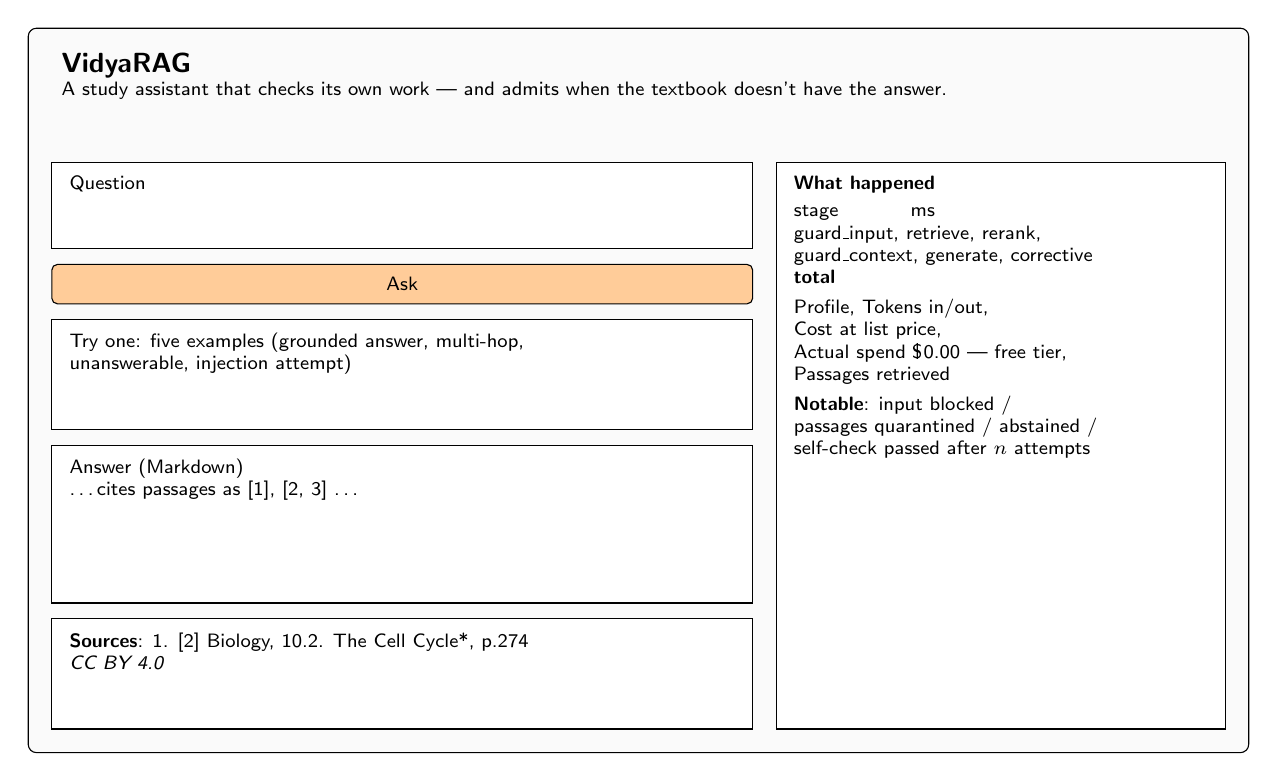
\begin{tikzpicture}[font=\sffamily\scriptsize]
\draw[rounded corners=3pt, fill=gray!4] (0,0) rectangle (15.5,9.2);
\node[anchor=north west, align=left] at (0.3,9.0) {\textbf{\normalsize VidyaRAG}\\A study assistant that checks its own work --- and admits when the textbook doesn't have the answer.};
\draw[fill=white] (0.3,6.4) rectangle (9.2,7.5); \node[anchor=north west] at (0.4,7.45) {Question};
\draw[fill=orange!40, rounded corners=2pt] (0.3,5.7) rectangle (9.2,6.2); \node at (4.75,5.95) {Ask};
\draw[fill=white] (0.3,4.1) rectangle (9.2,5.5); \node[anchor=north west, align=left] at (0.4,5.45) {Try one: five examples (grounded answer, multi-hop,\\ unanswerable, injection attempt)};
\draw[fill=white] (0.3,1.9) rectangle (9.2,3.9); \node[anchor=north west, align=left] at (0.4,3.85) {Answer (Markdown)\\\ldots cites passages as [1], [2, 3] \ldots};
\draw[fill=white] (0.3,0.3) rectangle (9.2,1.7); \node[anchor=north west, align=left] at (0.4,1.65) {\textbf{Sources}: 1. [2] Biology, 10.2. The Cell Cycle*, p.274\\ \textit{CC BY 4.0}};
\draw[fill=white] (9.5,0.3) rectangle (15.2,7.5); \node[anchor=north west, align=left] at (9.6,7.45) {\textbf{What happened}\\[2pt] stage \hfill ms\\ guard\_input, retrieve, rerank,\\ guard\_context, generate, corrective\\ \textbf{total}\\[3pt] Profile, Tokens in/out,\\ Cost at list price,\\ Actual spend \$0.00 --- free tier,\\ Passages retrieved\\[3pt] \textbf{Notable}: input blocked /\\ passages quarantined / abstained /\\ self-check passed after $n$ attempts};
\end{tikzpicture}
\caption{Layout built by \code{build_ui} \ev{app/app.py:158-194}: a question column (scale 3) and a trace column (scale 2).}
\label{fig:demo-layout}
\end{figure}

\subsection{How it works}

\begin{itemize}
  \item \textbf{Examples chosen to expose behaviour.} The five examples include a grounded question, a multi-hop question, \enquote{plausible, in-domain, and genuinely absent} (the oxytocin thresholds), and an injection attempt that \enquote{should be blocked before any retrieval happens} \ev{app/app.py:57-66}. The docstring's reason: \enquote{A demo where the failure modes are hard to trigger is a demo that only ever shows its best case.}
  \item \textbf{A single pipeline, configured through \code{Settings}.} \code{get_pipeline} builds the pipeline on first use and keeps it. It reads the profile from \code{Settings}, not \code{os.environ}; the docstring records the bug this fixed --- a local \code{VIDYARAG_PROFILE=baseline} in \code{.env} was honoured by the CLI and API and \enquote{silently ignored here} \ev{app/app.py:71-92}.
  \item \textbf{Every failure is shown, never a blank page.} \code{ask} catches any exception and displays \enquote{Something went wrong} with the exception's type and message \ev{app/app.py:147-155}.
  \item \textbf{The working is on screen.} \code{_render_trace} builds a stage table with a total, the profile, tokens, list price, \enquote{Actual spend \$0.00 --- free tier}, the number of passages retrieved, and notable events \ev{app/app.py:104-144}.
  \item \textbf{A formal GPU declaration.} ZeroGPU refuses to start a Space without an \code{@spaces.GPU} function, so one is declared inside a guarded import and never called; the comment explains that ZeroGPU is \enquote{the only Gradio hardware a free account may host} \ev{app/app.py:29-55}.
  \item \textbf{Launch settings.} \code{queue(max_size=16)}, port 7860, and server-side rendering disabled: a form with three Markdown panes \enquote{gains nothing from SSR and gains a second runtime that can fail on its own} \ev{app/app.py:197-208}.
\end{itemize}

\begin{background}[Gradio queueing]
With queueing enabled, Gradio processes each event listener with a default concurrency of one, so questions are answered one at a time; \code{max_size=16} caps how many can wait.
\end{background}

\begin{measured}[the live Space, exercised during this analysis]
The injection example was blocked end to end in under two seconds with zero tokens; the oxytocin example returned the abstention sentence; the anaphase and glucose examples returned cited answers, for example with the source \code{[2] Biology, 10.2. The Cell Cycle*, p.274}.
\end{measured}

\subsection{Demo findings}

\begin{enumerate}
  \item The \textbf{total} row over-reports time for every self-check answer, and the token and cost rows under-report (Sections~\ref{sec:latency-bug} and~\ref{sec:token-bug}). \tagV
  \item \textbf{Raw exception messages are shown to anonymous visitors.} This is convenient for debugging and discloses internal details such as exception types and upstream error text. \tagI
  \item \textbf{The Space's README quotes another profile's results.} It says the demo refuses 12 of 12 unanswerable questions, with recall 1.000 and precision 0.800 --- the \code{corrective} run's numbers. The Space runs \code{guarded}, whose committed run measured 11 of 12, recall 0.917 and precision 0.846 \ev{app/README\_space.md}. \tagV
  \item \textbf{\enquote{Self-check passed} is shown when the self-check did not run.} If grading fails, the policy accepts the draft, and \code{_render_trace} still prints \enquote{Self-check passed after 1 attempt(s)}, because it checks only that a corrective record exists and that the answer was not an abstention \ev{app/app.py:132-139}. A grading failure of exactly this kind occurred during this analysis (Section~\ref{sec:trace-failopen}). \tagV
  \item \textbf{No tests cover \code{app/app.py}.} \tagV
\end{enumerate}

\section{What each interface shows}

\begin{center}
\begin{tabularx}{\textwidth}{@{}>{\raggedright\arraybackslash}p{5.2cm}>{\centering\arraybackslash}X>{\centering\arraybackslash}X>{\centering\arraybackslash}X@{}}
\toprule
& \textbf{API} & \textbf{CLI \code{ask}} & \textbf{Demo}\\
\midrule
Answer text & \yes & \yes & \yes\\
Validated citations with licence & \yes & \yes & \yes\\
Passages used, with text & \yes & with \code{--context} (160 characters) & \no\\
Stage timings, tokens, list price & \yes & summary line & \yes\\
Abstention and guard events & \no & \no & \yes\\
Structured error codes & partly (503/422/500) & exit code 1 on \code{ValueError} & message only\\
\bottomrule
\end{tabularx}
\end{center}

\begin{recommended}
Either implement \code{book_slug} for \code{/v1/query} (the retrieval function already supports it) or remove it from the request model. Add \code{abstained} and \code{blocked} to \code{QueryResponse}, and make \code{grounded} false for guard refusals. Map upstream rate-limit and timeout errors to 429 and 503, and declare them in the OpenAPI schema. Correct the README's description of \code{/v1/search} and the Space README's numbers. In the demo, show a generic error message and log the details server-side.
\end{recommended}
